\documentclass[10pt,a4paper,danish]{article}
%% Indlæs ofte brugte pakker
\usepackage{amssymb}
\usepackage[danish]{babel}
\usepackage[utf8]{inputenc}
\usepackage{listings}
\usepackage{fancyhdr}
\usepackage{hyperref}
\usepackage{booktabs}
\usepackage{graphicx}
\usepackage{todonotes}
\usepackage{algorithmic}
\usepackage{amsmath}


\pagestyle{fancy}
\fancyhead{}
\fancyfoot{}
\rhead{\today}
\rfoot{\thepage}
\setlength{\parindent}{0pt}

% Opsæt indlæsning af filer
\lstset{
 language=Python,
 extendedchars=\true,
 inputencoding=utf8,
 linewidth=\textwidth, basicstyle=\small,
 numbers=left, numberstyle=\footnotesize,
 tabsize=2, showstringspaces=false,
 breaklines=true, breakatwhitespace=false,
}

%% Titel og forfatter
\title{G1\\Maskinarkitektur\\Efterår 2011}
\author{Jens Fredskov\\ Naja Mottelson (vsj465)\\Søren Pilgård (vpb984)}

%% Start dokumentet
\begin{document}

%% Vis titel
\maketitle
\newpage

%% Vis indholdsfortegnelse
\tableofcontents
\newpage

%% Klar, parat, start!
\section{Indledning}
Nærværende rapport tjener som dokumentation af gruppens arbejde med første
godkendelsesopgave. Vi har [Note to self! Antager vi!] løst og afprøvet samtlige
underopgaver. 

\section{g1-1}
På Figur \ref{fig:circ1} ses vores implementation af de grundlæggende logiske
gates vha. NAND-gates.

\begin{figure}[htb]
\begin{center}
\leavevmode
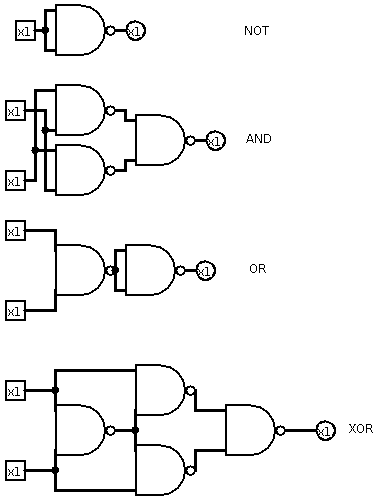
\includegraphics[scale=0.70]{circ1.png}
\end{center}
\caption{ALU, 4-bit}
\label{fig:circ1} 
\end{figure}

\section{g1-2}
Overordnet er vores 4-bit ALU (se Figur \ref{fig:circ2})implementeret som en serie af 4 1-bit ALU'er 
(se Figur \ref{fig:alu-1bit}. Hver 1-bit ALU indeholder (udover forskellige 
grundlæggende gates) en 1-bit adder, en multiplexer samt et modul til kontrol af overløb. 

\begin{figure}[htb]
\begin{center}
\leavevmode
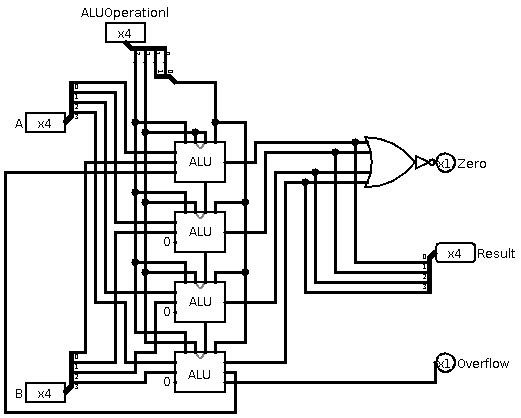
\includegraphics[scale=0.70]{circ2.png}
\end{center}
\caption{ALU, 4-bit}
\label{fig:circ2}
\end{figure}

\begin{figure}[htb]
\begin{center}
\leavevmode
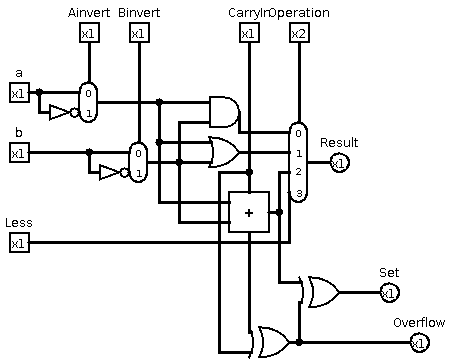
\includegraphics[scale=0.70]{alu-1bit-overflow.png}
\end{center}
\caption{1-bit ALU m. undersøgelse af overløb}
\label{fig:alu-1bit}
\end{figure}

\subsection{Multiplexer}

\begin{figure}[htb]
\begin{center}
\leavevmode
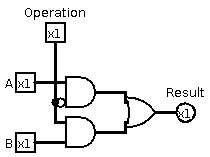
\includegraphics[scale=0.70]{mux-2bit.png}
\end{center}
\caption{MUX, 2 bit IN}
\label{fig:mux2bit} 
\end{figure}

\begin{figure}[htb]
\begin{center}
\leavevmode
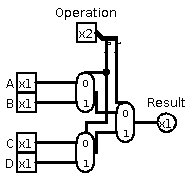
\includegraphics[scale=0.70]{mux-4bit.png}
\end{center}
\caption{MUX, 4 bit IN}
\label{fig:mux4bit} 
\end{figure}

\subsection{Adder}
\begin{figure}[htb]
\begin{center}
\leavevmode
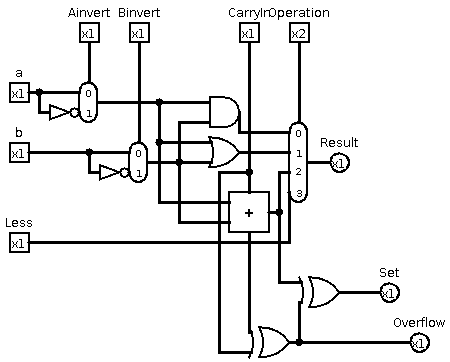
\includegraphics[scale=0.70]{adder-1bit.png}
\end{center}
\caption{}
\label{fig:adder}
\end{figure}

\subsection{Overløbskontrol}

\subsection{Adder}
\begin{figure}[htb]
\begin{center}
\leavevmode
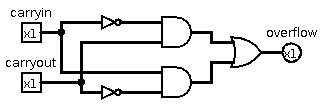
\includegraphics[scale=0.70]{overflow-detection.png}
\end{center}
\caption{}
\label{fig:overflow}
\end{figure}

\section{g1-3}


\end{document}
